% ============================================================
% B2-B2: ferromagnetic lock and two-stage Kondo screening
% ============================================================
\begin{frame}[t]
\ft{B2--B2: ferromagnetic lock, then two-stage Kondo}\par
\vspace{0.45cm}
\centering
% the figure sits at (0,0)-(5.83,6.0) in these units (y unit 0.9167cm = 5.5cm/6);
% each cartoon is at the height of the entropy plateau it explains.
% A blue halo around BOTH spins = one conduction channel (even, then odd) screening the pair.
\begin{tikzpicture}[x=1cm,y=0.9167cm,font=\footnotesize]
 \node[anchor=south west,inner sep=0] at (0,0) {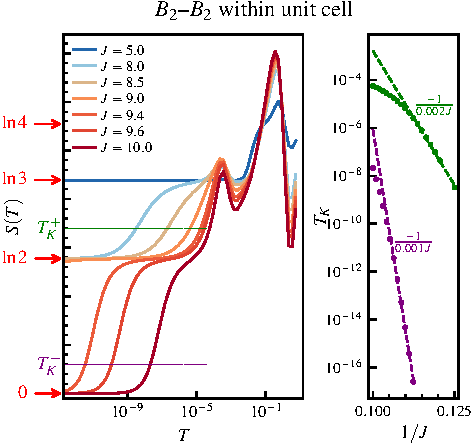
\includegraphics[height=5.5cm]{figures/jvsJsiteFM.pdf}};
 \path (-4.85,-0.45) rectangle (5.83,6.0);
 \node[anchor=north,font=\tiny,text=citegray] at (2.9,-0.05) {Two impurities on B2 sites of one unit cell. Right: both $T_K^\pm$ exponential in $1/J$};
 % ln 4: two free spins
 \foreach \x in {-1.25,-0.65}{\draw[cLM,fill=cLM!15,thick] (\x,4.32) circle (0.13);}
 \draw[->,cLM,>=stealth,line width=1.3pt] (-1.25,4.08)--(-1.25,4.56);
 \draw[->,cLM,>=stealth,line width=1.3pt] (-0.82,4.46)--(-0.48,4.18);
 \node[anchor=east] at (-1.95,4.32) {two free spins};
 % ln 3: locked into a spin 1
 \fill[cFM!30] (-0.95,3.50) ellipse (0.55 and 0.27); \draw[cFM] (-0.95,3.50) ellipse (0.55 and 0.27);
 \foreach \x in {-1.25,-0.65}{\draw[cLM,fill=cLM!15,thick] (\x,3.50) circle (0.13);
   \draw[->,cLM,>=stealth,line width=1.3pt] (\x,3.26)--(\x,3.74);}
 \node[anchor=east] at (-1.95,3.50) {\colorbox{cFM!30}{\mystrut FM lock: spin 1}};
 % ln 2: the even channel screens half of the spin 1
 \only<2->{
 \fill[cKondo!18] (-0.95,2.54) ellipse (0.72 and 0.40); \draw[cKondo,dashed] (-0.95,2.54) ellipse (0.72 and 0.40);
 \fill[cFM!30] (-0.95,2.54) ellipse (0.55 and 0.27); \draw[cFM] (-0.95,2.54) ellipse (0.55 and 0.27);
 \foreach \x in {-1.25,-0.65}{\draw[cLM,fill=cLM!15,thick] (\x,2.54) circle (0.13);
   \draw[->,cLM,>=stealth,line width=1.3pt] (\x,2.30)--(\x,2.78);}
 \node[anchor=east,align=right] at (-1.95,2.54) {\colorbox{cKondo!20}{\mystrut even channel screens}\\ below $T_K^+$: spin $\tfrac12$ left};
 }
 % 0: the odd channel screens the rest
 \only<3->{
 \fill[cKondo!18] (-0.95,0.72) ellipse (0.89 and 0.53); \draw[cKondo,dashed] (-0.95,0.72) ellipse (0.89 and 0.53);
 \fill[cKondo!32] (-0.95,0.72) ellipse (0.72 and 0.40); \draw[cKondo,dashed] (-0.95,0.72) ellipse (0.72 and 0.40);
 \fill[cFM!30] (-0.95,0.72) ellipse (0.55 and 0.27); \draw[cFM] (-0.95,0.72) ellipse (0.55 and 0.27);
 \foreach \x in {-1.25,-0.65}{\draw[cLM,fill=cLM!15,thick] (\x,0.72) circle (0.13);
   \draw[->,cLM,>=stealth,line width=1.3pt] (\x,0.48)--(\x,0.96);}
 \node[anchor=east,align=right] at (-1.95,0.72) {\colorbox{cKondo!20}{\mystrut odd channel screens}\\ below $T_K^-$: spin 0};
 }
\end{tikzpicture}\par
\onslide<3->{\tk{Ferromagnetic RKKY does not block Kondo screening: it splits it into two stages}}
\end{frame}
% Notes: The main result. Two impurities on the same unstacked sublattice: RKKY is ferromagnetic, and a ferromagnetic pair cannot screen itself.
% Notes: Read the entropy as before, a plateau at ln N means N states. ln 4: two free spins. ln 3: the spins have locked into a triplet, a spin 1 (J = 5: it stays there down to the lowest temperature).
% Notes: Larger J: the spin 1 is screened in two steps, one conduction channel at a time (the even and odd channels of the two-impurity NRG slide). Below T_K^+ the even channel screens half of the spin 1; a spin-1/2 is left: plateau at ln 2 (underscreened). It is NOT one impurity screened and the other free: the halo is around both. Below T_K^- the odd channel screens the rest: entropy 0.
% Notes: Right panel: both scales are Kondo scales, exponential in 1/J, with different exponents. T_K^- is many orders of magnitude below T_K^+: a very wide ln 2 plateau. As J grows the two scales approach each other.
% Notes: Contrast with A1-B2: there RKKY and Kondo are two ways to make a singlet. Here RKKY makes a bigger spin and Kondo then has to screen it twice.

% ============================================================
% B2-B2: distance dependence
% ============================================================
\begin{frame}[t]
\ft{Further apart: the two stages merge}
\vspace{0.4cm}
\begin{columns}[c]
\begin{column}{0.60\textwidth}
\centering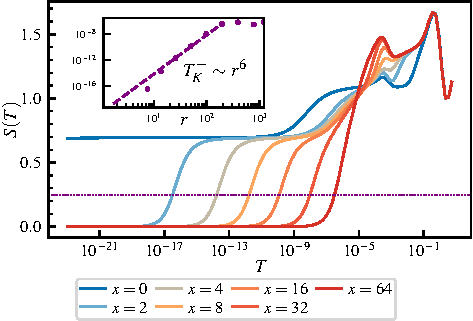
\includegraphics[width=\linewidth]{figures/jvsrsiteFM.pdf}\par
{\tiny\color{citegray} B2--B2 pairs, $x$ unit cells apart. Inset: $T_K^-$ against the distance $r$\par}
\vspace{0.4cm}
\onslide<2->{{\small\begin{tabular}{@{}l@{\ \ }l@{}}
 close pair: & \colorbox{cFM!30}{\mystrut wide $\ln 2$ plateau}, $T_K^-$ far below $T_K^+$\\[3pt]
 far apart: & $T_K^-\sim r^6$ catches up: \colorbox{cKondo!20}{\mystrut one Kondo scale}
\end{tabular}\par}}
\end{column}
\begin{column}{0.38\textwidth}
\onslide<3->{\centering\sitemap[0.85]{3}\\[4pt]\legend{3}\par}
\end{column}
\end{columns}
\end{frame}
% Notes: Move the two B2 impurities apart, same sublattice, x unit cells.
% Notes: Close pair (blue): the half-screened ln 2 plateau extends over many decades; T_K^- is out of the window at x = 0.
% Notes: Further apart the ferromagnetic RKKY weakens, T_K^- rises steeply, about r^6 (inset), until it reaches T_K^+. At x = 64 there is one crossover left: two independent single-impurity Kondo effects, the dilute limit.
% Notes: So two-stage screening is a property of close pairs.
% Notes: Site map complete: orange link = FM pair with two-stage screening.

